%--------------------
% Packages
% -------------------
\documentclass[11pt,a4paper]{article}
\usepackage[utf8]{inputenc}
\usepackage[T1]{fontenc}
%\usepackage{gentium}
\usepackage{mathptmx} % Use Times Font

\usepackage[pdftex]{graphicx} % Required for including pictures
\usepackage[english]{babel} % English translations
\usepackage[pdftex,linkcolor=black,pdfborder={0 0 0}]{hyperref} % Format links for pdf
\usepackage{calc} % To reset the counter in the document after title page
\usepackage{enumitem} % Includes lists
\usepackage{booktabs}
\usepackage{tabularx}
\usepackage{xcolor}
\usepackage{array}
\usepackage{tikz}
\usetikzlibrary{arrows.meta,positioning,fit,calc,shapes.multipart}

\frenchspacing % No double spacing between sentences
\linespread{1.2} % Set linespace
\usepackage[a4paper, lmargin=0.1666\paperwidth, rmargin=0.1666\paperwidth, tmargin=0.1111\paperheight, bmargin=0.1111\paperheight]{geometry} % margins
%\usepackage{parskip}

\usepackage[all]{nowidow} % Tries to remove widows
\usepackage[protrusion=true,expansion=true]{microtype} % Improves typography, load after fontpackage is selected

%-----------------------
% Set pdf information and add title, fill in the fields
%-----------------------
\hypersetup{
pdfsubject = {Wireless Sensor Networks Lab Group Project Proposal},
pdftitle = {WSN Lab Group Project Proposal Ideas},
pdfauthor = {Group 1}
}

%-----------------------
% Helper settings
%-----------------------
\setlist[itemize]{noitemsep, topsep=3pt}
\setlist[enumerate]{noitemsep, topsep=3pt}

\newcommand{\projecttitle}[1]{\subsection*{#1}}
\newcommand{\proposalbox}[1]{\vspace{0.3cm}\noindent\textbf{#1}\par\vspace{0.1cm}}

%-----------------------
% TikZ diagram styles
%-----------------------
\tikzset{
    nodebox/.style={
        draw,
        rounded corners,
        align=left,
        font=\small,
        inner sep=6pt,
        minimum width=3.4cm,
        fill=gray!6
    },
    gatewaybox/.style={
        draw,
        rounded corners,
        align=left,
        font=\small,
        inner sep=6pt,
        minimum width=3.7cm,
        fill=blue!6
    },
    functionbox/.style={
        draw,
        rounded corners,
        align=left,
        font=\small,
        inner sep=6pt,
        fill=green!6
    },
    packet/.style={
        -{Latex[length=2.2mm]},
        thick
    },
    downlink/.style={
        -{Latex[length=2.2mm]},
        thick,
        dashed
    },
    wireless/.style={
        -{Latex[length=2.2mm]},
        thick,
        dotted
    }
}


%-----------------------
% Begin document
%-----------------------
\begin{document}

\begin{center}
    {\LARGE \textbf{WSN Lab Group Project}}\\[0.3cm]
    {\large \textbf{Three Proposal Ideas}}\\[0.5cm]
    Group 1\\
    Wireless Sensor Networks Lab\\
    Proposal deadline: Friday, 15 May 2026
\end{center}

\vspace{0.8cm}

\section{Introduction}

The final group project should focus on low-power embedded devices and practical wireless communication between distributed sensor nodes. The system should collect sensor data, transmit it wirelessly to at least one central node or gateway, process the received data, and provide visualization, storage, or alerting. It should also include an experimental evaluation of aspects such as communication reliability, latency, range, scalability, or energy efficiency.

Our group already has a suitable technical foundation from the previous lab tasks. We have worked with IBR-Nodes running RIOT OS and implemented multi-node communication with a main node and several client nodes. The existing setup uses GNRC IPv6, UDP, \texttt{sock\_udp}, RPL, timers, shell commands, and different compile-time node roles. Therefore, the following proposals are designed to reuse and extend this foundation instead of starting from a completely new system.

The three proposed project ideas are:

\begin{enumerate}
    \item Smart Coaster WSN for Bar Table Monitoring
    \item Smart Greenhouse WSN with Wireless Irrigation Control
    \item Low-Power Environmental Safety Monitoring Network
\end{enumerate}

\section{Comparison of the Proposed Ideas}

\begin{table}[h]
    \centering
    \begin{tabularx}{\textwidth}{p{0.7cm} X p{2.7cm} p{2.4cm}}
        \toprule
        \textbf{Rank} & \textbf{Project Idea} & \textbf{Main Strength} & \textbf{Risk Level} \\
        \midrule
        1 & Smart Coaster WSN for Bar Table Monitoring
          & Original and strong live demo
          & Medium \\
        2 & Smart Greenhouse WSN with Wireless Irrigation Control
          & Strong sensor-actuator use case
          & Medium \\
        3 & Low-Power Environmental Safety Monitoring Network
          & Robust and easy to evaluate
          & Low \\
        \bottomrule
    \end{tabularx}
    \caption{Overview of the three recommended project proposals.}
\end{table}

\newpage

\section{Proposal 1: Smart Coaster WSN for Bar Table Monitoring}

\projecttitle{Project Title}

\textbf{Smart Coaster WSN: Low-Power Wireless Table Monitoring for Bars and Restaurants}

\projecttitle{Use Case and Motivation}

In a bar or restaurant, service staff often need to estimate when guests need new drinks, ice, or assistance. This project proposes a distributed wireless sensor network of smart coasters placed on tables. Each coaster acts as an embedded sensor node that measures the weight and temperature of a glass. From these measurements, the system estimates whether a glass is full, partially full, almost empty, or removed. A button on the coaster allows guests to call a waiter.

The collected data is transmitted wirelessly to a central gateway node representing the cash register or service station. The gateway processes incoming data and displays alerts such as a nearly empty glass, increasing drink temperature, or a waiter-call request.

\projecttitle{Objectives}

The main objectives are:

\begin{itemize}
    \item implement multiple embedded smart coaster nodes,
    \item collect weight, temperature, and button data,
    \item classify the glass state using threshold-based logic,
    \item transmit sensor data wirelessly to a central gateway,
    \item provide visualization or alerting at the gateway,
    \item evaluate reliability, latency, communication range, and energy-related trade-offs.
\end{itemize}

\projecttitle{Selected Wireless Technology}

The project will use IBR-Nodes running RIOT OS. Wireless communication will be implemented using IPv6/UDP over the GNRC network stack. RPL can be used to support multi-hop communication between coasters and the gateway. This directly builds on the previous multi-node setup with main and client node roles.

\projecttitle{Hardware Components}

Planned hardware components are:

\begin{itemize}
    \item 3--4 IBR-Nodes or comparable low-power embedded boards,
    \item load cell sensors with HX711 amplifiers for weight measurement,
    \item temperature sensors for drink or coaster temperature measurement,
    \item push buttons for waiter-call functionality,
    \item LEDs for local status indication,
    \item optional battery packs,
    \item one gateway node connected to a laptop for monitoring,
    \item optional relay node for multi-hop evaluation.
\end{itemize}

\projecttitle{System Architecture}

The system consists of several smart coaster nodes and one central gateway. Each coaster periodically samples its sensors and sends compact UDP messages to the gateway. The gateway stores the latest state of each coaster and derives alert states.

A possible message format is:

\begin{verbatim}
coaster:<node_id>:<seq>:<weight_g>:<temp_c_x10>:<button>:<glass_type>:<status>
\end{verbatim}

Example:

\begin{verbatim}
coaster:2:184:237:82:0:large:low
\end{verbatim}

This means that node 2 sent packet 184, measured 237 g, measured 8.2 degrees Celsius, the button was not pressed, the detected glass type is large, and the drink level is low.


\begin{figure}[h]
    \centering
    \resizebox{\textwidth}{!}{%
    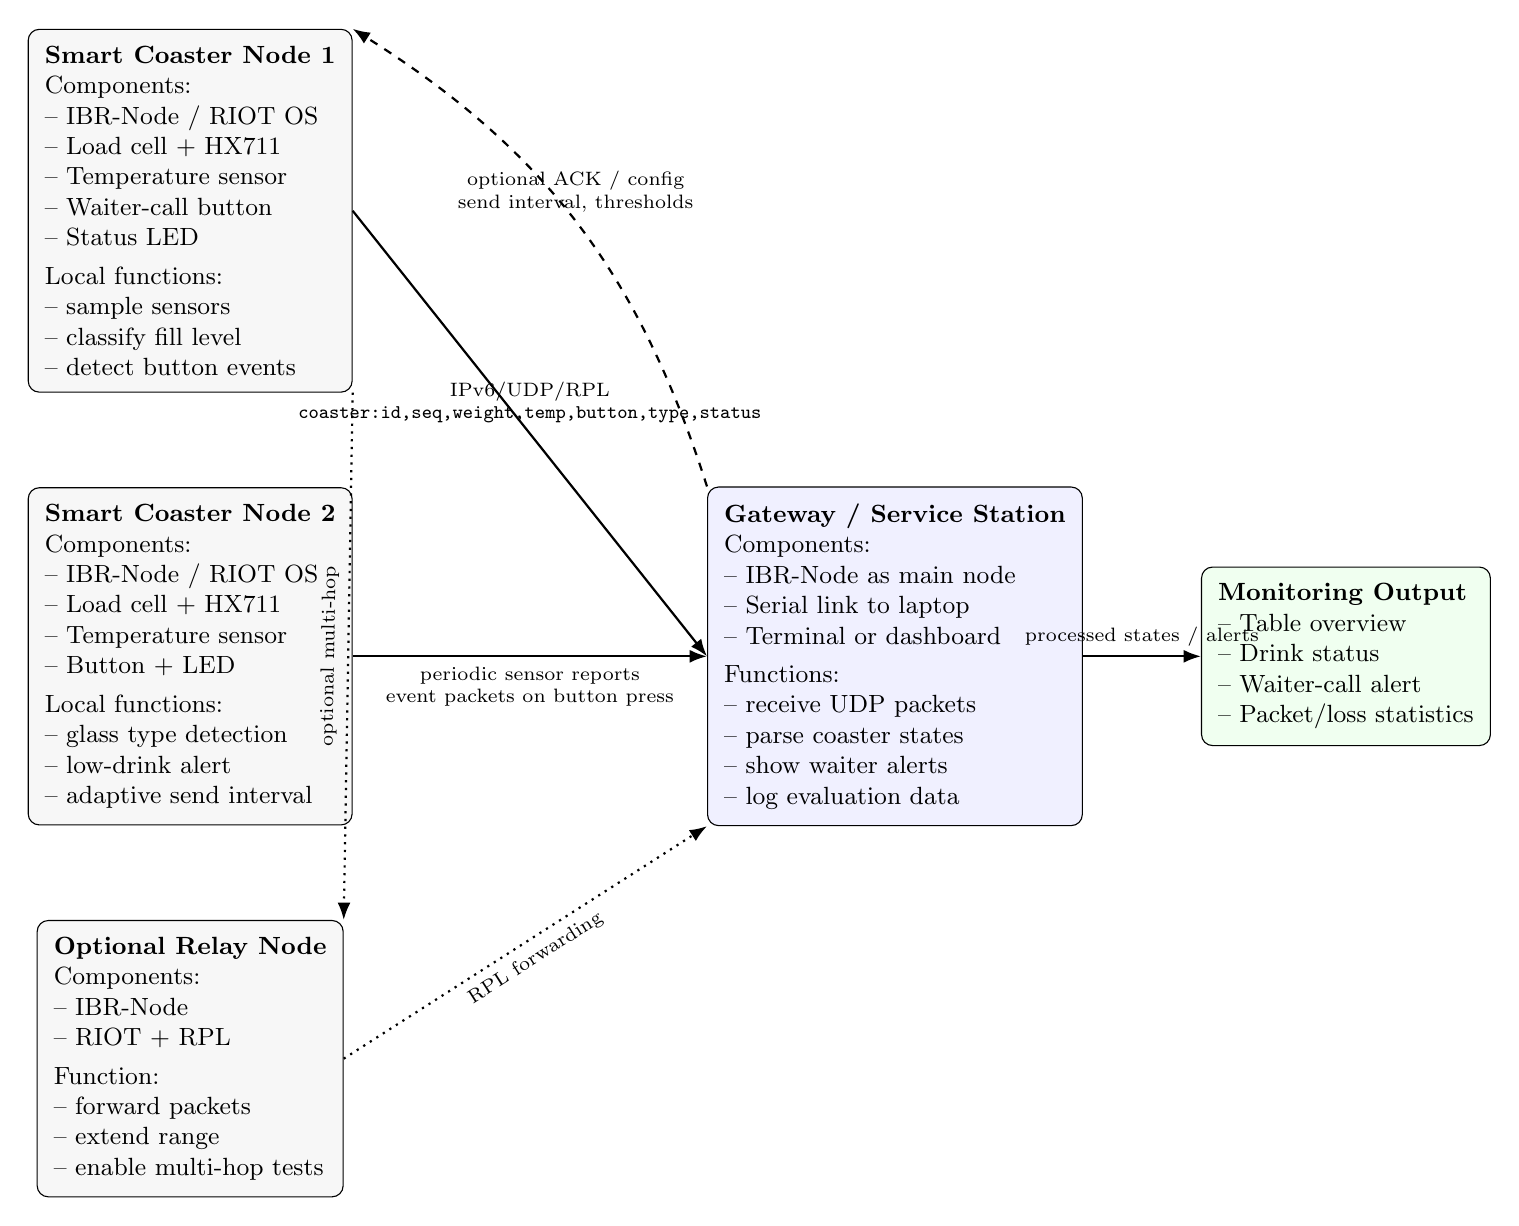
\begin{tikzpicture}[node distance=1.2cm and 1.8cm]
        \node[nodebox] (c1) {
            \textbf{Smart Coaster Node 1}\\
            Components:\\
            -- IBR-Node / RIOT OS\\
            -- Load cell + HX711\\
            -- Temperature sensor\\
            -- Waiter-call button\\
            -- Status LED\\[1mm]
            Local functions:\\
            -- sample sensors\\
            -- classify fill level\\
            -- detect button events
        };

        \node[nodebox, below=of c1] (c2) {
            \textbf{Smart Coaster Node 2}\\
            Components:\\
            -- IBR-Node / RIOT OS\\
            -- Load cell + HX711\\
            -- Temperature sensor\\
            -- Button + LED\\[1mm]
            Local functions:\\
            -- glass type detection\\
            -- low-drink alert\\
            -- adaptive send interval
        };

        \node[nodebox, below=of c2] (relay) {
            \textbf{Optional Relay Node}\\
            Components:\\
            -- IBR-Node\\
            -- RIOT + RPL\\[1mm]
            Function:\\
            -- forward packets\\
            -- extend range\\
            -- enable multi-hop tests
        };

        \node[gatewaybox, right=4.5cm of c2] (gw) {
            \textbf{Gateway / Service Station}\\
            Components:\\
            -- IBR-Node as main node\\
            -- Serial link to laptop\\
            -- Terminal or dashboard\\[1mm]
            Functions:\\
            -- receive UDP packets\\
            -- parse coaster states\\
            -- show waiter alerts\\
            -- log evaluation data
        };

        \node[functionbox, right=1.5cm of gw] (app) {
            \textbf{Monitoring Output}\\
            -- Table overview\\
            -- Drink status\\
            -- Waiter-call alert\\
            -- Packet/loss statistics
        };

        \draw[packet] (c1.east) -- node[above, align=center, font=\scriptsize] {
            IPv6/UDP/RPL\\
            \texttt{coaster:id,seq,weight,temp,button,type,status}
        } (gw.west);

        \draw[packet] (c2.east) -- node[below, align=center, font=\scriptsize] {
            periodic sensor reports\\
            event packets on button press
        } (gw.west);

        \draw[wireless] (c1.south east) -- node[above, sloped, font=\scriptsize] {optional multi-hop} (relay.north east);
        \draw[wireless] (relay.east) -- node[below, sloped, font=\scriptsize] {RPL forwarding} (gw.south west);

        \draw[packet] (gw.east) -- node[above, font=\scriptsize] {processed states / alerts} (app.west);
        \draw[downlink] (gw.north west) to[bend right=20] node[above, align=center, font=\scriptsize] {
            optional ACK / config\\
            send interval, thresholds
        } (c1.north east);
    \end{tikzpicture}
    }
    \caption{System architecture for the Smart Coaster WSN proposal.}
\end{figure}

\projecttitle{Minimum Functional Scope}

A minimal working system should include:

\begin{itemize}
    \item at least two smart coaster nodes,
    \item one gateway node,
    \item weight measurement,
    \item button event transmission,
    \item wireless sensor data transmission,
    \item gateway-side parsing and alert generation,
    \item basic terminal or dashboard output.
\end{itemize}

\projecttitle{Possible Extensions}

Possible extensions are:

\begin{itemize}
    \item temperature-based freshness or ice-melting indicator,
    \item distinction between two different glass types,
    \item multi-hop forwarding through an additional relay node,
    \item adaptive send intervals depending on glass state,
    \item simple acknowledgement mechanism for important events.
\end{itemize}

\projecttitle{Evaluation Plan}

The system can be evaluated using the following metrics:

\begin{itemize}
    \item \textbf{Packet delivery ratio:} received packets divided by sent packets.
    \item \textbf{Latency:} time between button press and visible gateway alert.
    \item \textbf{Sensor accuracy:} comparison between measured and expected glass states.
    \item \textbf{Range:} communication performance at different distances.
    \item \textbf{Energy efficiency:} comparison of different send intervals and event-based transmission.
\end{itemize}

\projecttitle{Live Demonstration}

The final demonstration shows several coasters on a table. A glass is placed on a coaster, filled or emptied, and the gateway updates the corresponding status. Pressing the service button triggers a waiter-call alert. Optionally, one coaster communicates via a relay node to demonstrate multi-hop communication.

\projecttitle{Assessment}

This is the strongest proposal because it is original, realistic, and directly suitable for a live demonstration. It combines sensing, wireless communication, gateway processing, alerting, and evaluation. The main risk is the mechanical calibration of the weight sensors.

\newpage

\section{Proposal 2: Smart Greenhouse WSN with Wireless Irrigation Control}

\projecttitle{Project Title}

\textbf{Smart Greenhouse WSN: Distributed Plant Monitoring and Wireless Irrigation Control}

\projecttitle{Use Case and Motivation}

Plants in a greenhouse or indoor environment require suitable moisture, temperature, humidity, and light conditions. Manual monitoring is inefficient, especially when multiple plants or zones are involved. This project proposes a wireless sensor network for monitoring several plant zones and optionally triggering irrigation or warning signals.

Each plant node measures environmental and soil conditions. The data is sent wirelessly to a gateway node. If a plant is too dry or the environment becomes unsuitable, the system generates an alert. Optionally, an actuator node can activate a small pump, LED, or fan.

\projecttitle{Objectives}

The main objectives are:

\begin{itemize}
    \item monitor multiple plant or greenhouse zones,
    \item collect soil moisture, temperature, humidity, and light data,
    \item transmit sensor values wirelessly to a gateway,
    \item classify plant state as normal, dry, too dark, or too warm,
    \item optionally control an actuator through wireless downlink commands,
    \item evaluate communication reliability, latency, and energy-efficiency trade-offs.
\end{itemize}

\projecttitle{Selected Wireless Technology}

The project will use low-power embedded nodes running RIOT OS. Communication will be based on IPv6/UDP. RPL can be used if multi-hop communication is needed, for example when one plant node cannot directly reach the gateway.

\projecttitle{Hardware Components}

Planned hardware components are:

\begin{itemize}
    \item 3--4 IBR-Nodes or comparable embedded boards,
    \item soil moisture sensors,
    \item temperature and humidity sensors,
    \item light sensors,
    \item optional water level sensor,
    \item optional small water pump or servo valve,
    \item optional LED or buzzer for local warnings,
    \item one gateway node connected to a monitoring laptop.
\end{itemize}

\projecttitle{System Architecture}

The system consists of multiple plant sensor nodes and one gateway node. Each plant node periodically measures local conditions and sends a sensor report. The gateway aggregates these reports and determines the state of each plant zone.

A possible message format is:

\begin{verbatim}
plant:<node_id>:<seq>:<soil>:<temp_c_x10>:<hum>:<light>:<status>
\end{verbatim}

Example:

\begin{verbatim}
plant:1:73:21:245:43:612:dry
\end{verbatim}

This means that plant node 1 sent packet 73, the soil moisture is low, the temperature is 24.5 degrees Celsius, the relative humidity is 43 percent, the light value is 612, and the state is dry.

If an actuator is included, the gateway can send downlink commands:

\begin{verbatim}
cmd:<node_id>:water:<duration_ms>
\end{verbatim}


\begin{figure}[h]
    \centering
    \resizebox{\textwidth}{!}{%
    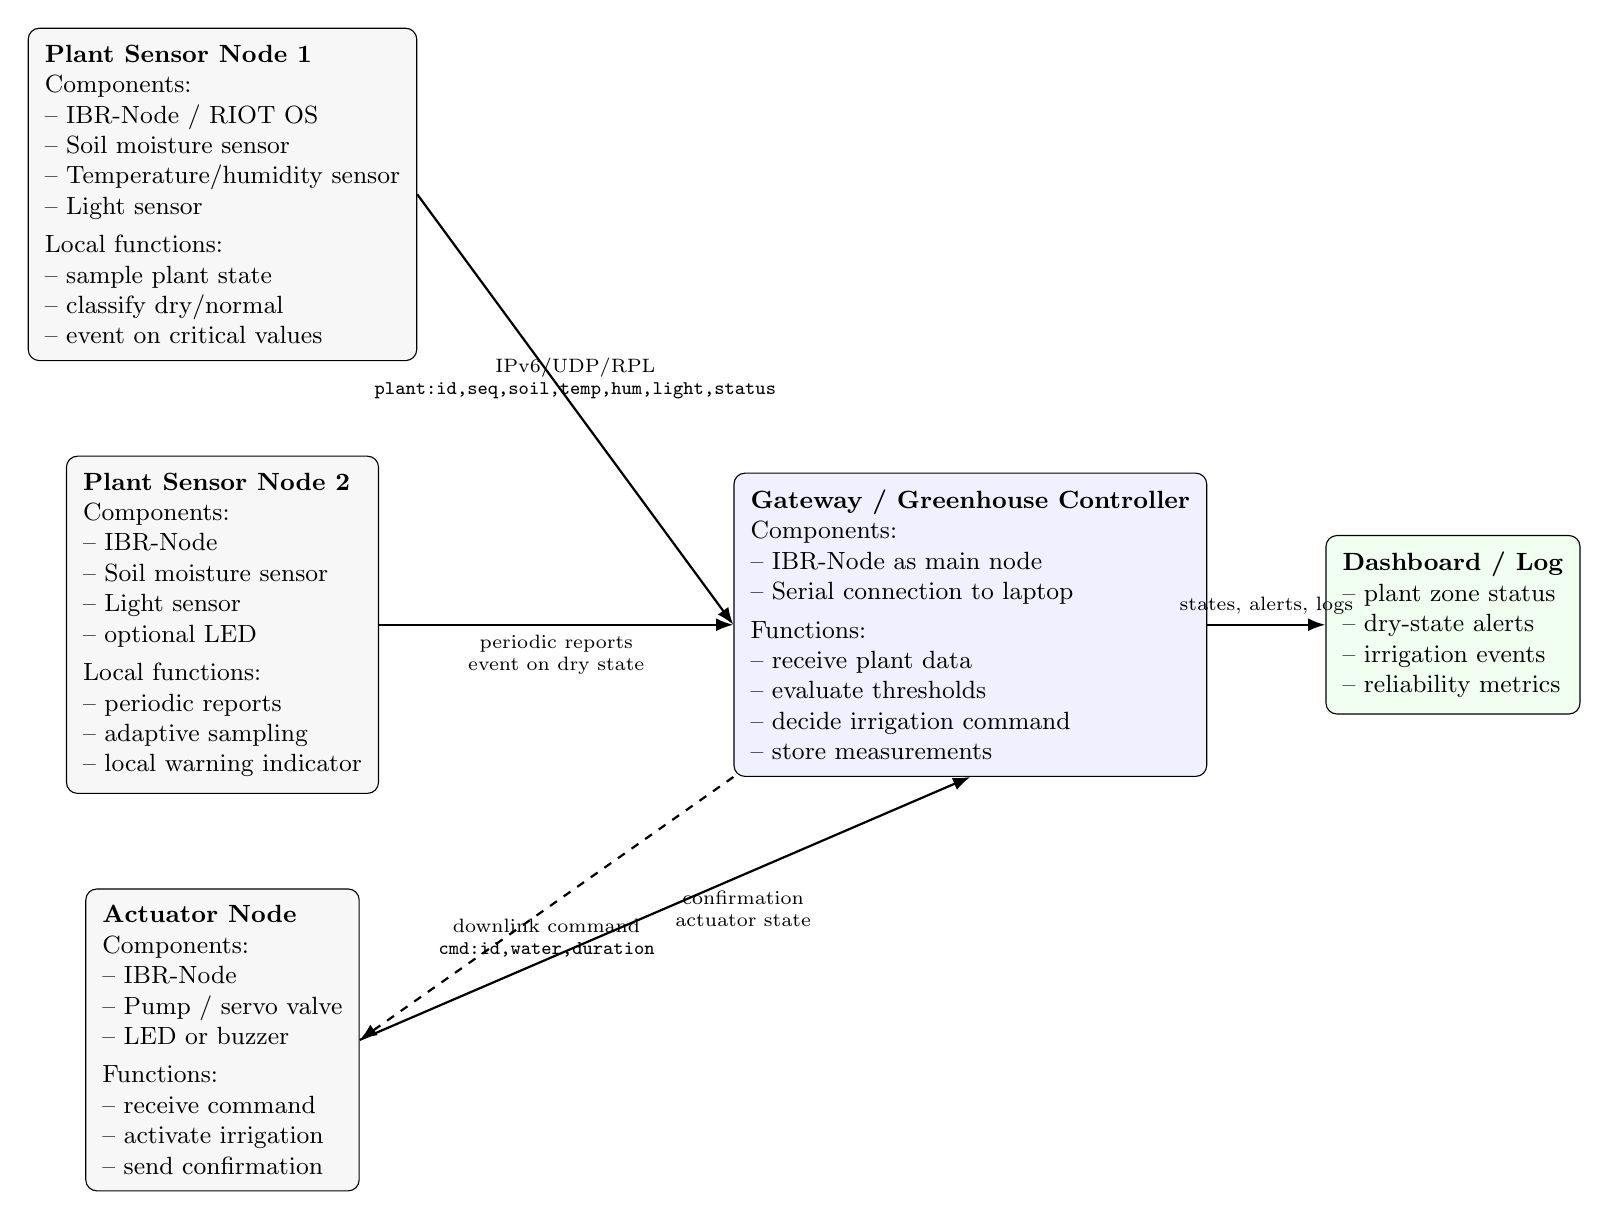
\begin{tikzpicture}[node distance=1.2cm and 1.8cm]
        \node[nodebox] (p1) {
            \textbf{Plant Sensor Node 1}\\
            Components:\\
            -- IBR-Node / RIOT OS\\
            -- Soil moisture sensor\\
            -- Temperature/humidity sensor\\
            -- Light sensor\\[1mm]
            Local functions:\\
            -- sample plant state\\
            -- classify dry/normal\\
            -- event on critical values
        };

        \node[nodebox, below=of p1] (p2) {
            \textbf{Plant Sensor Node 2}\\
            Components:\\
            -- IBR-Node\\
            -- Soil moisture sensor\\
            -- Light sensor\\
            -- optional LED\\[1mm]
            Local functions:\\
            -- periodic reports\\
            -- adaptive sampling\\
            -- local warning indicator
        };

        \node[nodebox, below=of p2] (act) {
            \textbf{Actuator Node}\\
            Components:\\
            -- IBR-Node\\
            -- Pump / servo valve\\
            -- LED or buzzer\\[1mm]
            Functions:\\
            -- receive command\\
            -- activate irrigation\\
            -- send confirmation
        };

        \node[gatewaybox, right=4.5cm of p2] (gw) {
            \textbf{Gateway / Greenhouse Controller}\\
            Components:\\
            -- IBR-Node as main node\\
            -- Serial connection to laptop\\[1mm]
            Functions:\\
            -- receive plant data\\
            -- evaluate thresholds\\
            -- decide irrigation command\\
            -- store measurements
        };

        \node[functionbox, right=1.5cm of gw] (dash) {
            \textbf{Dashboard / Log}\\
            -- plant zone status\\
            -- dry-state alerts\\
            -- irrigation events\\
            -- reliability metrics
        };

        \draw[packet] (p1.east) -- node[above, align=center, font=\scriptsize] {
            IPv6/UDP/RPL\\
            \texttt{plant:id,seq,soil,temp,hum,light,status}
        } (gw.west);

        \draw[packet] (p2.east) -- node[below, align=center, font=\scriptsize] {
            periodic reports\\
            event on dry state
        } (gw.west);

        \draw[downlink] (gw.south west) -- node[below, align=center, font=\scriptsize] {
            downlink command\\
            \texttt{cmd:id,water,duration}
        } (act.east);

        \draw[packet] (act.east) -- node[right, align=center, font=\scriptsize] {
            confirmation\\
            actuator state
        } (gw.south);

        \draw[packet] (gw.east) -- node[above, font=\scriptsize] {states, alerts, logs} (dash.west);
    \end{tikzpicture}
    }
    \caption{System architecture for the Smart Greenhouse WSN proposal.}
\end{figure}

\projecttitle{Minimum Functional Scope}

A minimal working system should include:

\begin{itemize}
    \item at least two plant sensor nodes,
    \item one gateway node,
    \item soil moisture measurement,
    \item temperature or light measurement,
    \item wireless sensor reports,
    \item gateway-side state classification,
    \item serial or dashboard visualization.
\end{itemize}

\projecttitle{Possible Extensions}

Possible extensions are:

\begin{itemize}
    \item automatic irrigation using a pump or valve,
    \item actuator confirmation messages,
    \item adaptive sampling based on plant state,
    \item multi-hop communication through a relay node,
    \item simple historical logging of plant conditions,
    \item comparison between periodic and event-driven communication.
\end{itemize}

\projecttitle{Evaluation Plan}

The system can be evaluated using:

\begin{itemize}
    \item \textbf{Packet delivery ratio:} reliability of periodic sensor reports.
    \item \textbf{Control latency:} time between dry-state detection and actuator command.
    \item \textbf{Sensor plausibility:} response to dry and wet soil conditions.
    \item \textbf{Range:} direct communication versus relayed communication.
    \item \textbf{Energy efficiency:} reduction of transmissions using adaptive sampling.
\end{itemize}

\projecttitle{Live Demonstration}

The live demonstration can use small plant pots or simulated soil conditions. A dry soil condition is created by removing the sensor from wet soil or using a dry sample. The plant node detects the dry condition and sends an alert to the gateway. The gateway displays the alert and optionally sends a command to activate a pump or LED.

\projecttitle{Assessment}

This proposal is strong because it naturally combines sensors and actuators. It is easy to explain, easy to demonstrate, and well aligned with WSN requirements. The main risk is handling water near electronics. This can be reduced by simulating the pump with an LED or using a controlled small water setup.

\newpage

\section{Proposal 3: Low-Power Environmental Safety Monitoring Network}

\projecttitle{Project Title}

\textbf{Low-Power Wireless Environmental Monitoring and Alert System}

\projecttitle{Use Case and Motivation}

Many rooms, laboratories, server rooms, and storage areas require continuous environmental monitoring. Temperature, humidity, light, air quality, or movement may indicate unsafe or undesirable conditions. This project proposes a distributed low-power wireless sensor network that monitors such parameters and reports warnings to a central gateway.

Compared to the other proposals, this idea is the most robust and technically safe. It is a classical WSN scenario and can be implemented even if actuator integration or mechanical sensor calibration becomes difficult.

\projecttitle{Objectives}

The main objectives are:

\begin{itemize}
    \item deploy multiple embedded environmental sensor nodes,
    \item collect temperature, humidity, light, air-quality, or motion data,
    \item transmit measurements wirelessly to a gateway,
    \item classify environmental state using thresholds,
    \item generate alerts for critical conditions,
    \item evaluate reliability, latency, range, scalability, and energy efficiency.
\end{itemize}

\projecttitle{Selected Wireless Technology}

The project will use IBR-Nodes or comparable low-power embedded boards. The nodes will communicate using IPv6/UDP over RIOT OS. RPL can be used to support multi-hop communication and evaluate scalability.

\projecttitle{Hardware Components}

Possible hardware components are:

\begin{itemize}
    \item 3--4 IBR-Nodes or comparable embedded boards,
    \item temperature and humidity sensors,
    \item light sensors,
    \item optional CO$_2$ or VOC sensor,
    \item optional PIR motion sensor,
    \item optional door/window contact,
    \item optional LED or buzzer as local alarm,
    \item one gateway node connected to a laptop.
\end{itemize}

\projecttitle{System Architecture}

The system consists of multiple environmental sensor nodes and a gateway. Each node periodically sends sensor reports. The gateway processes incoming values and determines whether a node is in a normal or warning state.

A possible message format is:

\begin{verbatim}
env:<node_id>:<seq>:<temp_c_x10>:<hum>:<light>:<motion>:<status>
\end{verbatim}

Example:

\begin{verbatim}
env:3:122:294:38:120:0:hot
\end{verbatim}

This means that node 3 sent packet 122, measured 29.4 degrees Celsius, 38 percent humidity, low light, no motion, and a hot-state warning.


\begin{figure}[h]
    \centering
    \resizebox{\textwidth}{!}{%
    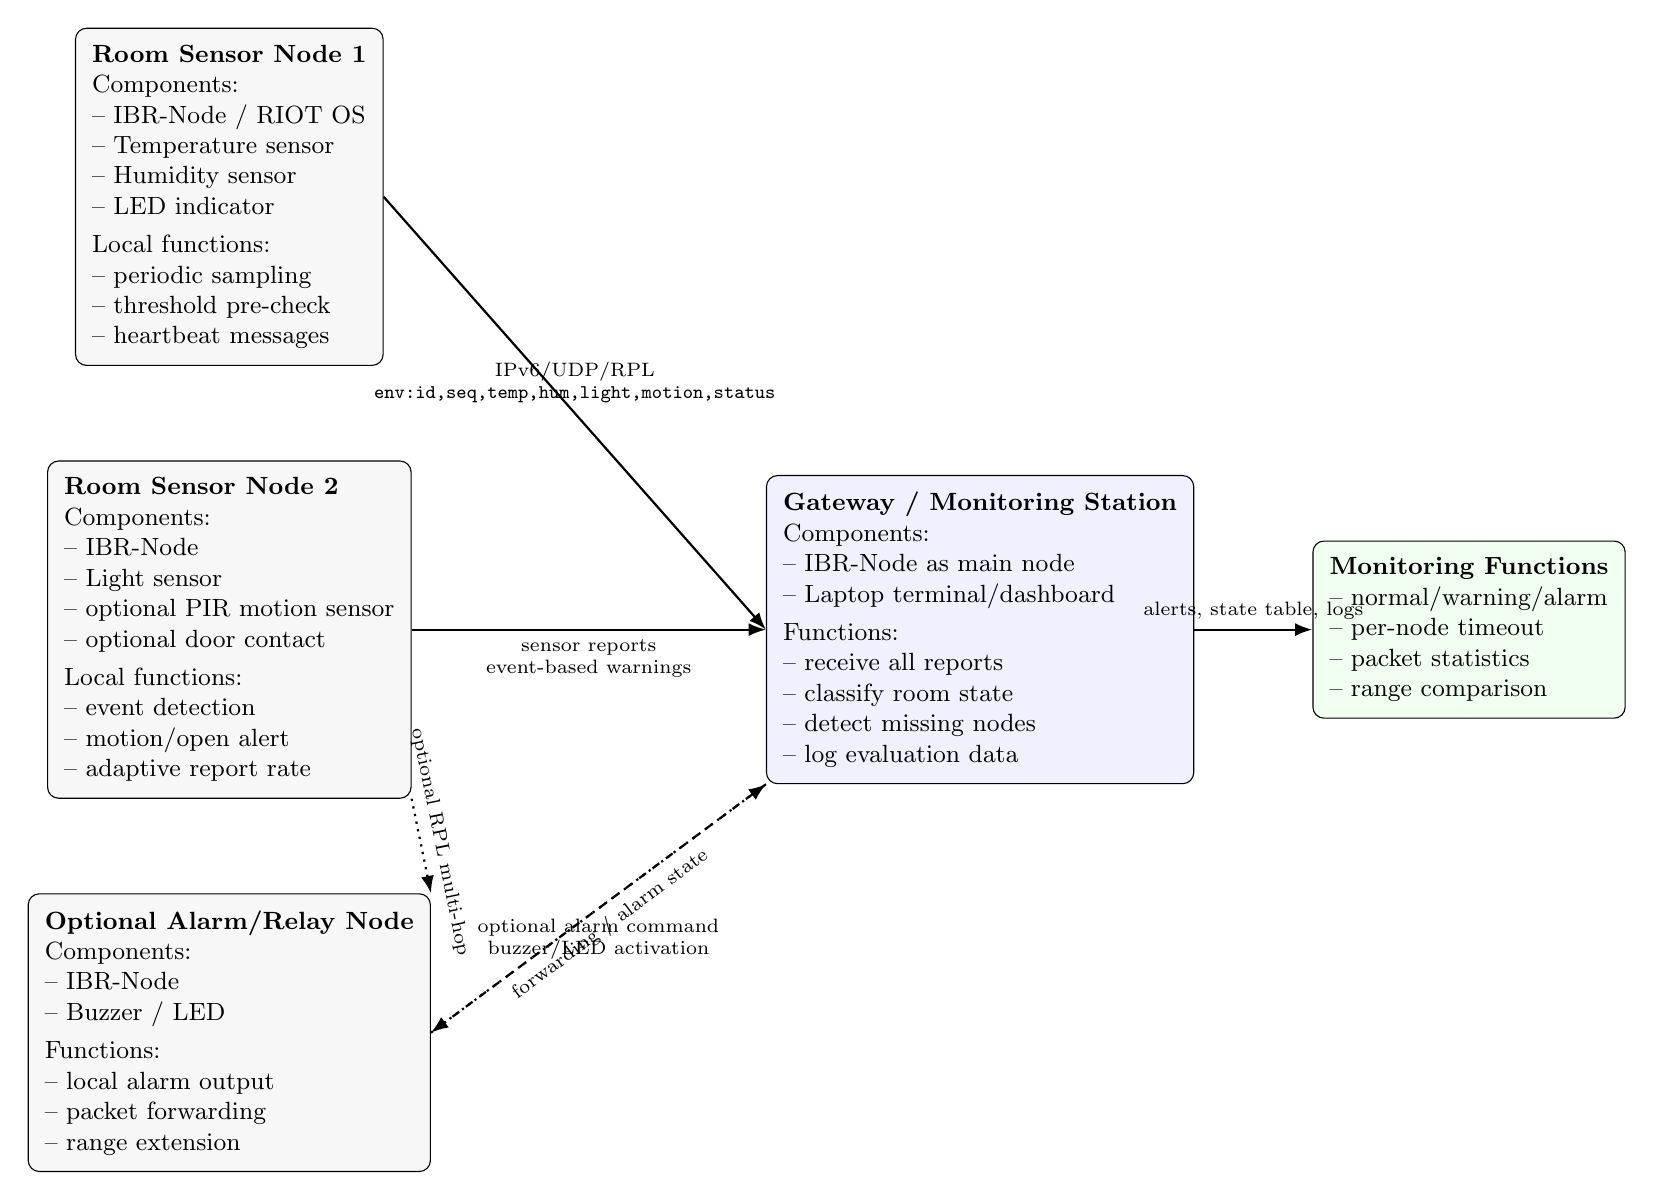
\begin{tikzpicture}[node distance=1.2cm and 1.8cm]
        \node[nodebox] (e1) {
            \textbf{Room Sensor Node 1}\\
            Components:\\
            -- IBR-Node / RIOT OS\\
            -- Temperature sensor\\
            -- Humidity sensor\\
            -- LED indicator\\[1mm]
            Local functions:\\
            -- periodic sampling\\
            -- threshold pre-check\\
            -- heartbeat messages
        };

        \node[nodebox, below=of e1] (e2) {
            \textbf{Room Sensor Node 2}\\
            Components:\\
            -- IBR-Node\\
            -- Light sensor\\
            -- optional PIR motion sensor\\
            -- optional door contact\\[1mm]
            Local functions:\\
            -- event detection\\
            -- motion/open alert\\
            -- adaptive report rate
        };

        \node[nodebox, below=of e2] (alarm) {
            \textbf{Optional Alarm/Relay Node}\\
            Components:\\
            -- IBR-Node\\
            -- Buzzer / LED\\[1mm]
            Functions:\\
            -- local alarm output\\
            -- packet forwarding\\
            -- range extension
        };

        \node[gatewaybox, right=4.5cm of e2] (gw) {
            \textbf{Gateway / Monitoring Station}\\
            Components:\\
            -- IBR-Node as main node\\
            -- Laptop terminal/dashboard\\[1mm]
            Functions:\\
            -- receive all reports\\
            -- classify room state\\
            -- detect missing nodes\\
            -- log evaluation data
        };

        \node[functionbox, right=1.5cm of gw] (mon) {
            \textbf{Monitoring Functions}\\
            -- normal/warning/alarm\\
            -- per-node timeout\\
            -- packet statistics\\
            -- range comparison
        };

        \draw[packet] (e1.east) -- node[above, align=center, font=\scriptsize] {
            IPv6/UDP/RPL\\
            \texttt{env:id,seq,temp,hum,light,motion,status}
        } (gw.west);

        \draw[packet] (e2.east) -- node[below, align=center, font=\scriptsize] {
            sensor reports\\
            event-based warnings
        } (gw.west);

        \draw[wireless] (e2.south east) -- node[above, sloped, font=\scriptsize] {optional RPL multi-hop} (alarm.north east);
        \draw[wireless] (alarm.east) -- node[below, sloped, font=\scriptsize] {forwarding / alarm state} (gw.south west);

        \draw[downlink] (gw.south west) -- node[below, align=center, font=\scriptsize] {
            optional alarm command\\
            buzzer/LED activation
        } (alarm.east);

        \draw[packet] (gw.east) -- node[above, font=\scriptsize] {alerts, state table, logs} (mon.west);
    \end{tikzpicture}
    }
    \caption{System architecture for the Environmental Safety Monitoring proposal.}
\end{figure}

\projecttitle{Minimum Functional Scope}

A minimal working system should include:

\begin{itemize}
    \item at least three environmental sensor nodes,
    \item one gateway node,
    \item temperature and humidity measurement,
    \item wireless transmission to the gateway,
    \item gateway-side threshold-based alert detection,
    \item terminal or dashboard visualization,
    \item basic communication evaluation.
\end{itemize}

\projecttitle{Possible Extensions}

Possible extensions are:

\begin{itemize}
    \item local alarm using buzzer or LEDs,
    \item adaptive reporting rate during critical states,
    \item motion-based event messages,
    \item multi-hop routing through a relay node,
    \item per-node timeout detection,
    \item historical logging and simple plots.
\end{itemize}

\projecttitle{Evaluation Plan}

The system can be evaluated using:

\begin{itemize}
    \item \textbf{Packet delivery ratio:} received reports versus expected reports.
    \item \textbf{Alert latency:} time between environmental change and gateway warning.
    \item \textbf{Range:} performance at different distances and through obstacles.
    \item \textbf{Scalability:} behavior with increasing number of reporting nodes.
    \item \textbf{Energy efficiency:} impact of different sampling and reporting intervals.
\end{itemize}

\projecttitle{Live Demonstration}

A live demo can simulate different environmental states. For example, one node is warmed by hand, another node is covered to reduce light, and a third node detects motion or a button event. The gateway displays the state of all nodes and highlights warnings. A relay node can be placed between sensor nodes and gateway to demonstrate multi-hop communication.

\projecttitle{Assessment}

This is the safest and most robust proposal. It is less original than the smart coaster idea but very well aligned with the WSN lab requirements. It also has low hardware risk because temperature, humidity, light, and motion sensors are common and easy to integrate.

\section{Final Recommendation}

The recommended primary proposal is the \textbf{Smart Coaster WSN}. It is the most original idea and provides a strong live demonstration. The \textbf{Smart Greenhouse WSN} is a strong second option because it naturally combines sensors and actuators. The \textbf{Environmental Safety Monitoring Network} is the safest fallback because it is technically robust and closely matches a classical wireless sensor network use case.

\begin{enumerate}
    \item \textbf{Smart Coaster WSN for Bar Table Monitoring}
    \item \textbf{Smart Greenhouse WSN with Wireless Irrigation Control}
    \item \textbf{Low-Power Environmental Safety Monitoring Network}
\end{enumerate}

\end{document}
